\documentclass[]{article}
\usepackage{lmodern}
\usepackage{amssymb,amsmath}
\usepackage{ifxetex,ifluatex}
\usepackage{fixltx2e} % provides \textsubscript
\ifnum 0\ifxetex 1\fi\ifluatex 1\fi=0 % if pdftex
  \usepackage[T1]{fontenc}
  \usepackage[utf8]{inputenc}
\else % if luatex or xelatex
  \ifxetex
    \usepackage{mathspec}
  \else
    \usepackage{fontspec}
  \fi
  \defaultfontfeatures{Ligatures=TeX,Scale=MatchLowercase}
\fi
% use upquote if available, for straight quotes in verbatim environments
\IfFileExists{upquote.sty}{\usepackage{upquote}}{}
% use microtype if available
\IfFileExists{microtype.sty}{%
\usepackage{microtype}
\UseMicrotypeSet[protrusion]{basicmath} % disable protrusion for tt fonts
}{}
\usepackage[margin=2.54cm]{geometry}
\usepackage{hyperref}
\hypersetup{unicode=true,
            pdftitle={Assignment 3: Physical Properties of Rivers},
            pdfauthor={Jake Greif},
            pdfborder={0 0 0},
            breaklinks=true}
\urlstyle{same}  % don't use monospace font for urls
\usepackage{color}
\usepackage{fancyvrb}
\newcommand{\VerbBar}{|}
\newcommand{\VERB}{\Verb[commandchars=\\\{\}]}
\DefineVerbatimEnvironment{Highlighting}{Verbatim}{commandchars=\\\{\}}
% Add ',fontsize=\small' for more characters per line
\usepackage{framed}
\definecolor{shadecolor}{RGB}{248,248,248}
\newenvironment{Shaded}{\begin{snugshade}}{\end{snugshade}}
\newcommand{\AlertTok}[1]{\textcolor[rgb]{0.94,0.16,0.16}{#1}}
\newcommand{\AnnotationTok}[1]{\textcolor[rgb]{0.56,0.35,0.01}{\textbf{\textit{#1}}}}
\newcommand{\AttributeTok}[1]{\textcolor[rgb]{0.77,0.63,0.00}{#1}}
\newcommand{\BaseNTok}[1]{\textcolor[rgb]{0.00,0.00,0.81}{#1}}
\newcommand{\BuiltInTok}[1]{#1}
\newcommand{\CharTok}[1]{\textcolor[rgb]{0.31,0.60,0.02}{#1}}
\newcommand{\CommentTok}[1]{\textcolor[rgb]{0.56,0.35,0.01}{\textit{#1}}}
\newcommand{\CommentVarTok}[1]{\textcolor[rgb]{0.56,0.35,0.01}{\textbf{\textit{#1}}}}
\newcommand{\ConstantTok}[1]{\textcolor[rgb]{0.00,0.00,0.00}{#1}}
\newcommand{\ControlFlowTok}[1]{\textcolor[rgb]{0.13,0.29,0.53}{\textbf{#1}}}
\newcommand{\DataTypeTok}[1]{\textcolor[rgb]{0.13,0.29,0.53}{#1}}
\newcommand{\DecValTok}[1]{\textcolor[rgb]{0.00,0.00,0.81}{#1}}
\newcommand{\DocumentationTok}[1]{\textcolor[rgb]{0.56,0.35,0.01}{\textbf{\textit{#1}}}}
\newcommand{\ErrorTok}[1]{\textcolor[rgb]{0.64,0.00,0.00}{\textbf{#1}}}
\newcommand{\ExtensionTok}[1]{#1}
\newcommand{\FloatTok}[1]{\textcolor[rgb]{0.00,0.00,0.81}{#1}}
\newcommand{\FunctionTok}[1]{\textcolor[rgb]{0.00,0.00,0.00}{#1}}
\newcommand{\ImportTok}[1]{#1}
\newcommand{\InformationTok}[1]{\textcolor[rgb]{0.56,0.35,0.01}{\textbf{\textit{#1}}}}
\newcommand{\KeywordTok}[1]{\textcolor[rgb]{0.13,0.29,0.53}{\textbf{#1}}}
\newcommand{\NormalTok}[1]{#1}
\newcommand{\OperatorTok}[1]{\textcolor[rgb]{0.81,0.36,0.00}{\textbf{#1}}}
\newcommand{\OtherTok}[1]{\textcolor[rgb]{0.56,0.35,0.01}{#1}}
\newcommand{\PreprocessorTok}[1]{\textcolor[rgb]{0.56,0.35,0.01}{\textit{#1}}}
\newcommand{\RegionMarkerTok}[1]{#1}
\newcommand{\SpecialCharTok}[1]{\textcolor[rgb]{0.00,0.00,0.00}{#1}}
\newcommand{\SpecialStringTok}[1]{\textcolor[rgb]{0.31,0.60,0.02}{#1}}
\newcommand{\StringTok}[1]{\textcolor[rgb]{0.31,0.60,0.02}{#1}}
\newcommand{\VariableTok}[1]{\textcolor[rgb]{0.00,0.00,0.00}{#1}}
\newcommand{\VerbatimStringTok}[1]{\textcolor[rgb]{0.31,0.60,0.02}{#1}}
\newcommand{\WarningTok}[1]{\textcolor[rgb]{0.56,0.35,0.01}{\textbf{\textit{#1}}}}
\usepackage{graphicx,grffile}
\makeatletter
\def\maxwidth{\ifdim\Gin@nat@width>\linewidth\linewidth\else\Gin@nat@width\fi}
\def\maxheight{\ifdim\Gin@nat@height>\textheight\textheight\else\Gin@nat@height\fi}
\makeatother
% Scale images if necessary, so that they will not overflow the page
% margins by default, and it is still possible to overwrite the defaults
% using explicit options in \includegraphics[width, height, ...]{}
\setkeys{Gin}{width=\maxwidth,height=\maxheight,keepaspectratio}
\IfFileExists{parskip.sty}{%
\usepackage{parskip}
}{% else
\setlength{\parindent}{0pt}
\setlength{\parskip}{6pt plus 2pt minus 1pt}
}
\setlength{\emergencystretch}{3em}  % prevent overfull lines
\providecommand{\tightlist}{%
  \setlength{\itemsep}{0pt}\setlength{\parskip}{0pt}}
\setcounter{secnumdepth}{0}
% Redefines (sub)paragraphs to behave more like sections
\ifx\paragraph\undefined\else
\let\oldparagraph\paragraph
\renewcommand{\paragraph}[1]{\oldparagraph{#1}\mbox{}}
\fi
\ifx\subparagraph\undefined\else
\let\oldsubparagraph\subparagraph
\renewcommand{\subparagraph}[1]{\oldsubparagraph{#1}\mbox{}}
\fi

%%% Use protect on footnotes to avoid problems with footnotes in titles
\let\rmarkdownfootnote\footnote%
\def\footnote{\protect\rmarkdownfootnote}

%%% Change title format to be more compact
\usepackage{titling}

% Create subtitle command for use in maketitle
\providecommand{\subtitle}[1]{
  \posttitle{
    \begin{center}\large#1\end{center}
    }
}

\setlength{\droptitle}{-2em}

  \title{Assignment 3: Physical Properties of Rivers}
    \pretitle{\vspace{\droptitle}\centering\huge}
  \posttitle{\par}
    \author{Jake Greif}
    \preauthor{\centering\large\emph}
  \postauthor{\par}
    \date{}
    \predate{}\postdate{}
  

\begin{document}
\maketitle

\hypertarget{overview}{%
\subsection{OVERVIEW}\label{overview}}

This exercise accompanies the lessons in Hydrologic Data Analysis on the
physical properties of rivers.

\hypertarget{directions}{%
\subsection{Directions}\label{directions}}

\begin{enumerate}
\def\labelenumi{\arabic{enumi}.}
\tightlist
\item
  Change ``Student Name'' on line 3 (above) with your name.
\item
  Work through the steps, \textbf{creating code and output} that fulfill
  each instruction.
\item
  Be sure to \textbf{answer the questions} in this assignment document.
\item
  When you have completed the assignment, \textbf{Knit} the text and
  code into a single PDF file.
\item
  After Knitting, submit the completed exercise (PDF file) to the
  dropbox in Sakai. Add your last name into the file name (e.g.,
  ``Salk\_A03\_RiversPhysical.Rmd'') prior to submission.
\end{enumerate}

The completed exercise is due on 18 September 2019 at 9:00 am.

\hypertarget{setup}{%
\subsection{Setup}\label{setup}}

\begin{enumerate}
\def\labelenumi{\arabic{enumi}.}
\tightlist
\item
  Verify your working directory is set to the R project file,
\item
  Load the tidyverse, dataRetrieval, and cowplot packages
\item
  Set your ggplot theme (can be theme\_classic or something else)
\item
  Import a data frame called ``MysterySiteDischarge'' from USGS gage
  site 03431700. Upload all discharge data for the entire period of
  record. Rename columns 4 and 5 as ``Discharge'' and ``Approval.Code''.
  DO NOT LOOK UP WHERE THIS SITE IS LOCATED.
\item
  Build a ggplot of discharge over the entire period of record.
\end{enumerate}

\begin{Shaded}
\begin{Highlighting}[]
\CommentTok{# Check Working Directory}
\KeywordTok{getwd}\NormalTok{()}
\end{Highlighting}
\end{Shaded}

\begin{verbatim}
## [1] "/Users/jakegreif/Duke/Fall_2019/Hydrologic_Data_Analysis"
\end{verbatim}

\begin{Shaded}
\begin{Highlighting}[]
\CommentTok{# Load Packages}
\KeywordTok{library}\NormalTok{(tidyverse)}
\KeywordTok{library}\NormalTok{(dataRetrieval)}
\KeywordTok{library}\NormalTok{(cowplot)}
\KeywordTok{library}\NormalTok{(lubridate)}

\CommentTok{# Import Data}
\NormalTok{MysterySiteDischarge <-}\StringTok{ }\KeywordTok{readNWISdv}\NormalTok{(}\DataTypeTok{siteNumbers =} \StringTok{"03431700"}\NormalTok{,}
                     \DataTypeTok{parameterCd =} \StringTok{"00060"}\NormalTok{,}
                     \DataTypeTok{startDate =} \StringTok{""}\NormalTok{,}
                     \DataTypeTok{endDate =} \StringTok{""}\NormalTok{)}

\KeywordTok{names}\NormalTok{(MysterySiteDischarge)[}\DecValTok{4}\OperatorTok{:}\DecValTok{5}\NormalTok{] <-}\StringTok{ }\KeywordTok{c}\NormalTok{(}\StringTok{"Discharge"}\NormalTok{, }\StringTok{"Approval.Code"}\NormalTok{)}

\CommentTok{# Set ggplot Theme}
\NormalTok{mytheme <-}\StringTok{ }\KeywordTok{theme_classic}\NormalTok{()}

\KeywordTok{theme_set}\NormalTok{(mytheme)}

\CommentTok{# Discharge over entire period}
\NormalTok{MystPlot <-}\StringTok{ }
\StringTok{  }\KeywordTok{ggplot}\NormalTok{(MysterySiteDischarge, }\KeywordTok{aes}\NormalTok{(}\DataTypeTok{x =}\NormalTok{ Date, }\DataTypeTok{y =}\NormalTok{ Discharge)) }\OperatorTok{+}
\StringTok{         }\KeywordTok{geom_line}\NormalTok{() }\OperatorTok{+}
\StringTok{         }\KeywordTok{xlab}\NormalTok{(}\StringTok{"Year"}\NormalTok{)}
\KeywordTok{print}\NormalTok{(MystPlot)}
\end{Highlighting}
\end{Shaded}

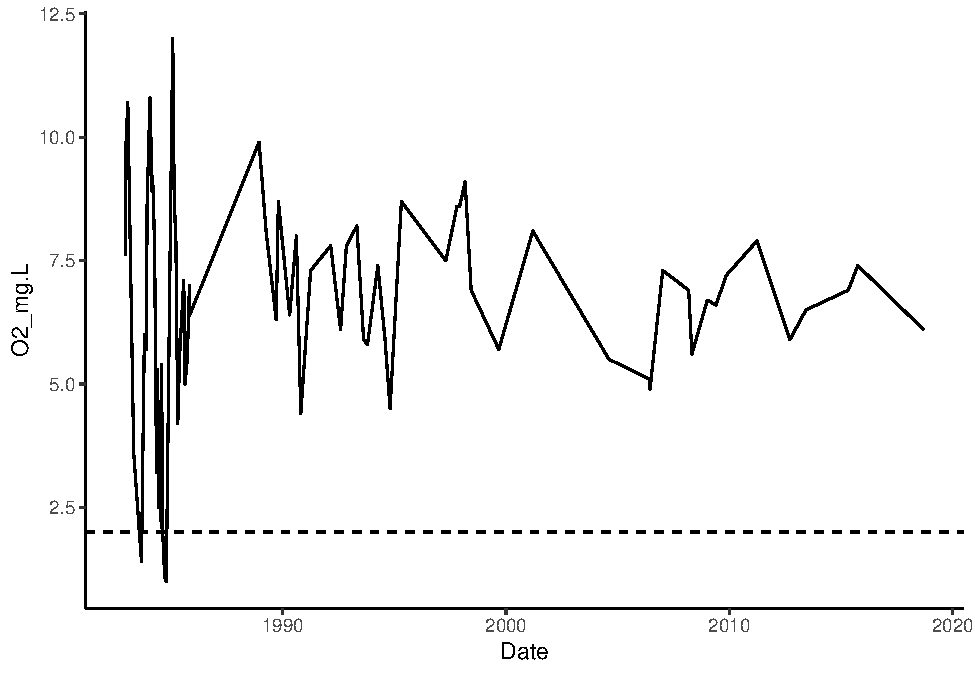
\includegraphics{A03_RiversPhysical_files/figure-latex/unnamed-chunk-1-1.pdf}

\hypertarget{analyze-seasonal-patterns-in-discharge}{%
\subsection{Analyze seasonal patterns in
discharge}\label{analyze-seasonal-patterns-in-discharge}}

\begin{enumerate}
\def\labelenumi{\arabic{enumi}.}
\setcounter{enumi}{4}
\tightlist
\item
  Add a ``Year'' and ``Day.of.Year'' column to the data frame.
\item
  Create a new data frame called ``MysterySiteDischarge.Pattern'' that
  has columns for Day.of.Year, median discharge for a given day of year,
  75th percentile discharge for a given day of year, and 25th percentile
  discharge for a given day of year. Hint: the summarise function
  includes \texttt{quantile}, wherein you must specify \texttt{probs} as
  a value between 0 and 1.
\item
  Create a plot of median, 75th quantile, and 25th quantile discharges
  against day of year. Median should be black, other lines should be
  gray.
\end{enumerate}

\begin{Shaded}
\begin{Highlighting}[]
\CommentTok{# Add Year column}
\NormalTok{MysterySiteDischarge <-}\StringTok{ }
\StringTok{  }\NormalTok{MysterySiteDischarge }\OperatorTok
\StringTok{  }\KeywordTok{mutate}\NormalTok{(}\DataTypeTok{Year =} \KeywordTok{year}\NormalTok{(Date))}

\CommentTok{# Add Day.of.Year column}
\NormalTok{MysterySiteDischarge <-}\StringTok{ }\KeywordTok{mutate}\NormalTok{(MysterySiteDischarge, }
                                         \DataTypeTok{DOY =} \KeywordTok{yday}\NormalTok{(Date))}

\CommentTok{# Calculate median discharge, create columns for 25th/75th percentiles}
\NormalTok{MysterySiteDischarge.Pattern <-}\StringTok{ }\NormalTok{MysterySiteDischarge }\OperatorTok
\StringTok{  }\KeywordTok{group_by}\NormalTok{(DOY) }\OperatorTok
\StringTok{  }\KeywordTok{summarise}\NormalTok{(}\DataTypeTok{Median.Discharge =} \KeywordTok{median}\NormalTok{(Discharge), }
            \DataTypeTok{Discharge.75th =} \KeywordTok{quantile}\NormalTok{(Discharge, }\DataTypeTok{probs =} \FloatTok{0.75}\NormalTok{),}
            \DataTypeTok{Discharge.25th =} \KeywordTok{quantile}\NormalTok{(Discharge, }\DataTypeTok{probs =} \FloatTok{0.25}\NormalTok{))}

\CommentTok{# Create plot of median, 75th/25th quantiles}
\NormalTok{MysteryPatternPlot <-}\StringTok{ }
\StringTok{  }\KeywordTok{ggplot}\NormalTok{(MysterySiteDischarge.Pattern, }\KeywordTok{aes}\NormalTok{(}\DataTypeTok{x =}\NormalTok{ DOY)) }\OperatorTok{+}
\StringTok{  }\KeywordTok{geom_line}\NormalTok{(}\KeywordTok{aes}\NormalTok{(}\DataTypeTok{y =}\NormalTok{ Median.Discharge)) }\OperatorTok{+}
\StringTok{  }\KeywordTok{geom_line}\NormalTok{(}\KeywordTok{aes}\NormalTok{(}\DataTypeTok{y =}\NormalTok{ Discharge}\FloatTok{.75}\NormalTok{th), }\DataTypeTok{color =} \StringTok{"gray"}\NormalTok{) }\OperatorTok{+}
\StringTok{  }\KeywordTok{geom_line}\NormalTok{(}\KeywordTok{aes}\NormalTok{(}\DataTypeTok{y =}\NormalTok{ Discharge}\FloatTok{.25}\NormalTok{th), }\DataTypeTok{color =} \StringTok{"gray"}\NormalTok{) }\OperatorTok{+}\StringTok{  }
\StringTok{  }\KeywordTok{labs}\NormalTok{(}\DataTypeTok{x =} \StringTok{"Day of Year"}\NormalTok{, }\DataTypeTok{y =} \KeywordTok{expression}\NormalTok{(}\StringTok{"Discharge (ft"}\OperatorTok{^}\DecValTok{3}\OperatorTok{*}\StringTok{"/s)"}\NormalTok{))}
\KeywordTok{print}\NormalTok{(MysteryPatternPlot)}
\end{Highlighting}
\end{Shaded}

\includegraphics{A03_RiversPhysical_files/figure-latex/unnamed-chunk-2-1.pdf}

\begin{enumerate}
\def\labelenumi{\arabic{enumi}.}
\setcounter{enumi}{7}
\tightlist
\item
  What seasonal patterns do you see? What does this tell you about
  precipitation patterns and climate in the watershed?
\end{enumerate}

\begin{quote}
The mystery river has relatively high flow during the winter months, and
discharge is noticably lower throughout the summer and fall. The
discharge only noticeably increases again around October/November. This
river must be in a region that primarily has winter precipitation, and a
dry summer.
\end{quote}

\hypertarget{create-and-analyze-recurrence-intervals}{%
\subsection{Create and analyze recurrence
intervals}\label{create-and-analyze-recurrence-intervals}}

\begin{enumerate}
\def\labelenumi{\arabic{enumi}.}
\setcounter{enumi}{8}
\tightlist
\item
  Create two separate data frames for MysterySite.Annual.30yr (first 30
  years of record) and MysterySite.Annual.Full (all years of record).
  Use a pipe to create your new data frame(s) that includes the year,
  the peak discharge observed in that year, a ranking of peak
  discharges, the recurrence interval, and the exceedende probability.
\end{enumerate}

\begin{Shaded}
\begin{Highlighting}[]
\CommentTok{# Create MysterySite.Annual.30yr data frame}
\NormalTok{MysterySite.Annual}\FloatTok{.30}\NormalTok{yr <-}\StringTok{ }
\StringTok{  }\NormalTok{MysterySiteDischarge }\OperatorTok
\StringTok{  }\KeywordTok{filter}\NormalTok{(Year }\OperatorTok{<}\StringTok{ }\DecValTok{1996}\NormalTok{) }\OperatorTok
\StringTok{  }\KeywordTok{group_by}\NormalTok{(Year) }\OperatorTok
\StringTok{  }\KeywordTok{summarise}\NormalTok{(}\DataTypeTok{PeakDischarge =} \KeywordTok{max}\NormalTok{(Discharge)) }\OperatorTok\StringTok{ }
\StringTok{  }\KeywordTok{mutate}\NormalTok{(}\DataTypeTok{Rank =} \KeywordTok{rank}\NormalTok{(}\OperatorTok{-}\NormalTok{PeakDischarge), }
         \DataTypeTok{RecurrenceInterval =}\NormalTok{ (}\KeywordTok{length}\NormalTok{(Year) }\OperatorTok{+}\StringTok{ }\DecValTok{1}\NormalTok{)}\OperatorTok{/}\NormalTok{Rank, }
         \DataTypeTok{Probability =} \DecValTok{1}\OperatorTok{/}\NormalTok{RecurrenceInterval)}

\CommentTok{# Create MysterySite.Annual.Full data frame}
\NormalTok{MysterySite.Annual.Full <-}\StringTok{ }
\StringTok{  }\NormalTok{MysterySiteDischarge }\OperatorTok
\StringTok{  }\KeywordTok{group_by}\NormalTok{(Year) }\OperatorTok
\StringTok{  }\KeywordTok{summarise}\NormalTok{(}\DataTypeTok{PeakDischarge =} \KeywordTok{max}\NormalTok{(Discharge)) }\OperatorTok\StringTok{ }
\StringTok{  }\KeywordTok{mutate}\NormalTok{(}\DataTypeTok{Rank =} \KeywordTok{rank}\NormalTok{(}\OperatorTok{-}\NormalTok{PeakDischarge), }
         \DataTypeTok{RecurrenceInterval =}\NormalTok{ (}\KeywordTok{length}\NormalTok{(Year) }\OperatorTok{+}\StringTok{ }\DecValTok{1}\NormalTok{)}\OperatorTok{/}\NormalTok{Rank, }
         \DataTypeTok{Probability =} \DecValTok{1}\OperatorTok{/}\NormalTok{RecurrenceInterval)}
\end{Highlighting}
\end{Shaded}

\begin{enumerate}
\def\labelenumi{\arabic{enumi}.}
\setcounter{enumi}{9}
\tightlist
\item
  Create a plot that displays the discharge vs.~recurrence interval
  relationship for the two separate data frames (one set of points
  includes the values computed from the first 30 years of the record and
  the other set of points includes the values computed for all years of
  the record.
\end{enumerate}

\begin{Shaded}
\begin{Highlighting}[]
\CommentTok{# Create discharge vs. recurrence interval plots}
\NormalTok{MystRecurrencePlot.Combined <-}\StringTok{ }
\StringTok{  }\KeywordTok{ggplot}\NormalTok{(MysterySite.Annual.Full,}
         \KeywordTok{aes}\NormalTok{(}\DataTypeTok{x =}\NormalTok{ RecurrenceInterval, }\DataTypeTok{y =}\NormalTok{ PeakDischarge)) }\OperatorTok{+}
\StringTok{  }\KeywordTok{geom_point}\NormalTok{() }\OperatorTok{+}
\StringTok{  }\KeywordTok{geom_point}\NormalTok{(}\DataTypeTok{data =}\NormalTok{ MysterySite.Annual}\FloatTok{.30}\NormalTok{yr, }\DataTypeTok{color =} \StringTok{"#02818a"}\NormalTok{,}
             \KeywordTok{aes}\NormalTok{(}\DataTypeTok{x =}\NormalTok{ RecurrenceInterval, }\DataTypeTok{y =}\NormalTok{ PeakDischarge)) }\OperatorTok{+}
\StringTok{  }\KeywordTok{scale_y_log10}\NormalTok{()}
\KeywordTok{print}\NormalTok{(MystRecurrencePlot.Combined)}
\end{Highlighting}
\end{Shaded}

\includegraphics{A03_RiversPhysical_files/figure-latex/unnamed-chunk-4-1.pdf}

\begin{enumerate}
\def\labelenumi{\arabic{enumi}.}
\setcounter{enumi}{10}
\tightlist
\item
  Create a model to predict the discharge for a 100-year flood for both
  sets of recurrence intervals.
\end{enumerate}

\begin{Shaded}
\begin{Highlighting}[]
\CommentTok{# 30yr model}
\NormalTok{Myst.RImodel}\FloatTok{.30}\NormalTok{yr <-}\StringTok{ }\KeywordTok{lm}\NormalTok{(}\DataTypeTok{data =}\NormalTok{ MysterySite.Annual}\FloatTok{.30}\NormalTok{yr, PeakDischarge }\OperatorTok{~}\StringTok{ }\KeywordTok{log}\NormalTok{(RecurrenceInterval))}
\KeywordTok{summary}\NormalTok{(Myst.RImodel}\FloatTok{.30}\NormalTok{yr)}
\end{Highlighting}
\end{Shaded}

\begin{verbatim}
## 
## Call:
## lm(formula = PeakDischarge ~ log(RecurrenceInterval), data = MysterySite.Annual.30yr)
## 
## Residuals:
##     Min      1Q  Median      3Q     Max 
## -974.12 -337.65   34.84  232.57 2908.00 
## 
## Coefficients:
##                         Estimate Std. Error t value Pr(>|t|)    
## (Intercept)               -69.87     185.73  -0.376     0.71    
## log(RecurrenceInterval)  1217.79     147.16   8.275 5.26e-09 ***
## ---
## Signif. codes:  0 '***' 0.001 '**' 0.01 '*' 0.05 '.' 0.1 ' ' 1
## 
## Residual standard error: 673.9 on 28 degrees of freedom
## Multiple R-squared:  0.7098, Adjusted R-squared:  0.6994 
## F-statistic: 68.48 on 1 and 28 DF,  p-value: 5.261e-09
\end{verbatim}

\begin{Shaded}
\begin{Highlighting}[]
\NormalTok{Myst.RImodel}\FloatTok{.30}\NormalTok{yr}\OperatorTok{$}\NormalTok{coefficients}
\end{Highlighting}
\end{Shaded}

\begin{verbatim}
##             (Intercept) log(RecurrenceInterval) 
##               -69.87363              1217.79015
\end{verbatim}

\begin{Shaded}
\begin{Highlighting}[]
\NormalTok{Myst.RImodel}\FloatTok{.30}\NormalTok{yr}\OperatorTok{$}\NormalTok{coefficients[}\DecValTok{1}\NormalTok{] }\OperatorTok{+}\StringTok{ }\NormalTok{Myst.RImodel}\FloatTok{.30}\NormalTok{yr}\OperatorTok{$}\NormalTok{coefficients[}\DecValTok{2}\NormalTok{]}\OperatorTok{*}\KeywordTok{log}\NormalTok{(}\DecValTok{100}\NormalTok{)}
\end{Highlighting}
\end{Shaded}

\begin{verbatim}
## (Intercept) 
##    5538.257
\end{verbatim}

\begin{Shaded}
\begin{Highlighting}[]
\CommentTok{# Full model}
\NormalTok{Myst.RImodel.Full <-}\StringTok{ }\KeywordTok{lm}\NormalTok{(}\DataTypeTok{data =}\NormalTok{ MysterySite.Annual.Full, PeakDischarge }\OperatorTok{~}\StringTok{ }\KeywordTok{log}\NormalTok{(RecurrenceInterval))}
\KeywordTok{summary}\NormalTok{(Myst.RImodel.Full)}
\end{Highlighting}
\end{Shaded}

\begin{verbatim}
## 
## Call:
## lm(formula = PeakDischarge ~ log(RecurrenceInterval), data = MysterySite.Annual.Full)
## 
## Residuals:
##     Min      1Q  Median      3Q     Max 
## -955.95 -236.29   41.91  210.67 2805.35 
## 
## Coefficients:
##                         Estimate Std. Error t value Pr(>|t|)    
## (Intercept)               -2.001    116.322  -0.017    0.986    
## log(RecurrenceInterval) 1052.234     88.834  11.845   <2e-16 ***
## ---
## Signif. codes:  0 '***' 0.001 '**' 0.01 '*' 0.05 '.' 0.1 ' ' 1
## 
## Residual standard error: 578.3 on 52 degrees of freedom
## Multiple R-squared:  0.7296, Adjusted R-squared:  0.7244 
## F-statistic: 140.3 on 1 and 52 DF,  p-value: < 2.2e-16
\end{verbatim}

\begin{Shaded}
\begin{Highlighting}[]
\NormalTok{Myst.RImodel.Full}\OperatorTok{$}\NormalTok{coefficients}
\end{Highlighting}
\end{Shaded}

\begin{verbatim}
##             (Intercept) log(RecurrenceInterval) 
##               -2.000535             1052.234166
\end{verbatim}

\begin{Shaded}
\begin{Highlighting}[]
\NormalTok{Myst.RImodel.Full}\OperatorTok{$}\NormalTok{coefficients[}\DecValTok{1}\NormalTok{] }\OperatorTok{+}\StringTok{ }\NormalTok{Myst.RImodel.Full}\OperatorTok{$}\NormalTok{coefficients[}\DecValTok{2}\NormalTok{]}\OperatorTok{*}\KeywordTok{log}\NormalTok{(}\DecValTok{100}\NormalTok{)}
\end{Highlighting}
\end{Shaded}

\begin{verbatim}
## (Intercept) 
##    4843.717
\end{verbatim}

\begin{enumerate}
\def\labelenumi{\arabic{enumi}.}
\setcounter{enumi}{11}
\tightlist
\item
  How did the recurrence interval plots and predictions of a 100-year
  flood differ among the two data frames? What does this tell you about
  the stationarity of discharge in this river?
\end{enumerate}

\begin{quote}
The 30 year recurrence interval plot is steeper and the 100-year flood
prediction is greater than the recurrence interval and 100-year flood
discharge derived from the full dataset. Overall, the first 30 years saw
higher discharges compared to the full dataset, and therefore using only
the first 30 years would cause one to over-estimate the discharge of
certain flood events. This tells us that the discharge of the river is
not stationary.
\end{quote}

\hypertarget{reflection}{%
\subsection{Reflection}\label{reflection}}

\begin{enumerate}
\def\labelenumi{\arabic{enumi}.}
\setcounter{enumi}{12}
\tightlist
\item
  What are 2-3 conclusions or summary points about river discharge you
  learned through your analysis?
\end{enumerate}

\begin{quote}
The timing and magnitude of discharge in rivers across the country are
highly dependent on climate and precipitation, but both timing and
magnitude do not stay constant. They change are changing with a changing
climate and precipitation patterns, therefore the idea of stationarity
does not apply well to many rivers.
\end{quote}

\begin{enumerate}
\def\labelenumi{\arabic{enumi}.}
\setcounter{enumi}{13}
\tightlist
\item
  What data, visualizations, and/or models supported your conclusions
  from 13?
\end{enumerate}

\begin{quote}
Observing the mean discharge on each day of the year over the course of
data collection period made it easier to identify seasonal trends in
discharge. Also, comapring the recurrence intervals of the first 30
years vs.~the full data set tested the assumption of stationarity.
\end{quote}

\begin{enumerate}
\def\labelenumi{\arabic{enumi}.}
\setcounter{enumi}{14}
\tightlist
\item
  Did hands-on data analysis impact your learning about discharge
  relative to a theory-based lesson? If so, how?
\end{enumerate}

\begin{quote}
Yes, but I think it would have been a little more difficult to grasp
some concepts without a theory-based background. Being able to
manipulate the data myself allowed me to get familiar with it at my own
pace, and I was able to think about why the data is the way it is by
comparing it to my prior theory-based lessons.
\end{quote}

\begin{enumerate}
\def\labelenumi{\arabic{enumi}.}
\setcounter{enumi}{15}
\tightlist
\item
  How did the real-world data compare with your expectations from
  theory?
\end{enumerate}

\begin{quote}
Finding that the 30 year recurrence intervals did not match up with the
full data recurrence intervals was technically surprising. However, when
I initially learned the theory, I was taught then that stationarity was
dead. So, while the results were what I expected, compared to
traditional theory that assumes there is stationarity, these results are
surprising.
\end{quote}


\end{document}
